21. \begin{figure}[ht!]
\center{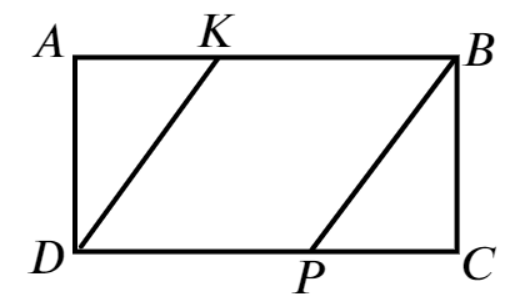
\includegraphics[scale=0.35]{g8-21.png}}
\end{figure}\\
$AK=\cfrac{3}{8}AB=\cfrac{3}{8}\cdot8=3\Rightarrow KB=8-3=5,$ аналогично $DP=5,$ значит в четырёхугольнике $KBPD$ противоположные стороны параллельны и равны, поэтому он является параллелограммом. Также по теореме Пифагора $KD=\sqrt{AK^2+AD^2}=\sqrt{9+16}=5,$ аналогично $BP=5,$ поэтому $KBPD$ является ромбом. Его периметр равен $4\cdot5=20,$ а площадь равна $BC\cdot DP=4\cdot5=20.$\\
